\documentclass[]{article}
\usepackage{lmodern}
\usepackage{amssymb,amsmath}
\usepackage{ifxetex,ifluatex}
\usepackage{fixltx2e} % provides \textsubscript
\ifnum 0\ifxetex 1\fi\ifluatex 1\fi=0 % if pdftex
  \usepackage[T1]{fontenc}
  \usepackage[utf8]{inputenc}
\else % if luatex or xelatex
  \ifxetex
    \usepackage{mathspec}
  \else
    \usepackage{fontspec}
  \fi
  \defaultfontfeatures{Ligatures=TeX,Scale=MatchLowercase}
\fi
% use upquote if available, for straight quotes in verbatim environments
\IfFileExists{upquote.sty}{\usepackage{upquote}}{}
% use microtype if available
\IfFileExists{microtype.sty}{%
\usepackage{microtype}
\UseMicrotypeSet[protrusion]{basicmath} % disable protrusion for tt fonts
}{}
\usepackage[margin=1in]{geometry}
\usepackage{hyperref}
\hypersetup{unicode=true,
            pdftitle={R Notebook},
            pdfborder={0 0 0},
            breaklinks=true}
\urlstyle{same}  % don't use monospace font for urls
\usepackage{color}
\usepackage{fancyvrb}
\newcommand{\VerbBar}{|}
\newcommand{\VERB}{\Verb[commandchars=\\\{\}]}
\DefineVerbatimEnvironment{Highlighting}{Verbatim}{commandchars=\\\{\}}
% Add ',fontsize=\small' for more characters per line
\usepackage{framed}
\definecolor{shadecolor}{RGB}{248,248,248}
\newenvironment{Shaded}{\begin{snugshade}}{\end{snugshade}}
\newcommand{\KeywordTok}[1]{\textcolor[rgb]{0.13,0.29,0.53}{\textbf{#1}}}
\newcommand{\DataTypeTok}[1]{\textcolor[rgb]{0.13,0.29,0.53}{#1}}
\newcommand{\DecValTok}[1]{\textcolor[rgb]{0.00,0.00,0.81}{#1}}
\newcommand{\BaseNTok}[1]{\textcolor[rgb]{0.00,0.00,0.81}{#1}}
\newcommand{\FloatTok}[1]{\textcolor[rgb]{0.00,0.00,0.81}{#1}}
\newcommand{\ConstantTok}[1]{\textcolor[rgb]{0.00,0.00,0.00}{#1}}
\newcommand{\CharTok}[1]{\textcolor[rgb]{0.31,0.60,0.02}{#1}}
\newcommand{\SpecialCharTok}[1]{\textcolor[rgb]{0.00,0.00,0.00}{#1}}
\newcommand{\StringTok}[1]{\textcolor[rgb]{0.31,0.60,0.02}{#1}}
\newcommand{\VerbatimStringTok}[1]{\textcolor[rgb]{0.31,0.60,0.02}{#1}}
\newcommand{\SpecialStringTok}[1]{\textcolor[rgb]{0.31,0.60,0.02}{#1}}
\newcommand{\ImportTok}[1]{#1}
\newcommand{\CommentTok}[1]{\textcolor[rgb]{0.56,0.35,0.01}{\textit{#1}}}
\newcommand{\DocumentationTok}[1]{\textcolor[rgb]{0.56,0.35,0.01}{\textbf{\textit{#1}}}}
\newcommand{\AnnotationTok}[1]{\textcolor[rgb]{0.56,0.35,0.01}{\textbf{\textit{#1}}}}
\newcommand{\CommentVarTok}[1]{\textcolor[rgb]{0.56,0.35,0.01}{\textbf{\textit{#1}}}}
\newcommand{\OtherTok}[1]{\textcolor[rgb]{0.56,0.35,0.01}{#1}}
\newcommand{\FunctionTok}[1]{\textcolor[rgb]{0.00,0.00,0.00}{#1}}
\newcommand{\VariableTok}[1]{\textcolor[rgb]{0.00,0.00,0.00}{#1}}
\newcommand{\ControlFlowTok}[1]{\textcolor[rgb]{0.13,0.29,0.53}{\textbf{#1}}}
\newcommand{\OperatorTok}[1]{\textcolor[rgb]{0.81,0.36,0.00}{\textbf{#1}}}
\newcommand{\BuiltInTok}[1]{#1}
\newcommand{\ExtensionTok}[1]{#1}
\newcommand{\PreprocessorTok}[1]{\textcolor[rgb]{0.56,0.35,0.01}{\textit{#1}}}
\newcommand{\AttributeTok}[1]{\textcolor[rgb]{0.77,0.63,0.00}{#1}}
\newcommand{\RegionMarkerTok}[1]{#1}
\newcommand{\InformationTok}[1]{\textcolor[rgb]{0.56,0.35,0.01}{\textbf{\textit{#1}}}}
\newcommand{\WarningTok}[1]{\textcolor[rgb]{0.56,0.35,0.01}{\textbf{\textit{#1}}}}
\newcommand{\AlertTok}[1]{\textcolor[rgb]{0.94,0.16,0.16}{#1}}
\newcommand{\ErrorTok}[1]{\textcolor[rgb]{0.64,0.00,0.00}{\textbf{#1}}}
\newcommand{\NormalTok}[1]{#1}
\usepackage{graphicx,grffile}
\makeatletter
\def\maxwidth{\ifdim\Gin@nat@width>\linewidth\linewidth\else\Gin@nat@width\fi}
\def\maxheight{\ifdim\Gin@nat@height>\textheight\textheight\else\Gin@nat@height\fi}
\makeatother
% Scale images if necessary, so that they will not overflow the page
% margins by default, and it is still possible to overwrite the defaults
% using explicit options in \includegraphics[width, height, ...]{}
\setkeys{Gin}{width=\maxwidth,height=\maxheight,keepaspectratio}
\IfFileExists{parskip.sty}{%
\usepackage{parskip}
}{% else
\setlength{\parindent}{0pt}
\setlength{\parskip}{6pt plus 2pt minus 1pt}
}
\setlength{\emergencystretch}{3em}  % prevent overfull lines
\providecommand{\tightlist}{%
  \setlength{\itemsep}{0pt}\setlength{\parskip}{0pt}}
\setcounter{secnumdepth}{0}
% Redefines (sub)paragraphs to behave more like sections
\ifx\paragraph\undefined\else
\let\oldparagraph\paragraph
\renewcommand{\paragraph}[1]{\oldparagraph{#1}\mbox{}}
\fi
\ifx\subparagraph\undefined\else
\let\oldsubparagraph\subparagraph
\renewcommand{\subparagraph}[1]{\oldsubparagraph{#1}\mbox{}}
\fi

%%% Use protect on footnotes to avoid problems with footnotes in titles
\let\rmarkdownfootnote\footnote%
\def\footnote{\protect\rmarkdownfootnote}

%%% Change title format to be more compact
\usepackage{titling}

% Create subtitle command for use in maketitle
\newcommand{\subtitle}[1]{
  \posttitle{
    \begin{center}\large#1\end{center}
    }
}

\setlength{\droptitle}{-2em}
  \title{R Notebook}
  \pretitle{\vspace{\droptitle}\centering\huge}
  \posttitle{\par}
  \author{}
  \preauthor{}\postauthor{}
  \date{}
  \predate{}\postdate{}


\begin{document}
\maketitle

How exactly did Donald Trump surprise the world and became the President
of US? Let us take a look at what is it that he said to the people of US
that appealed the most to them.

I will perform a sentiment analysis of all the 56 speeches Trump gave
across US en route to the Oval office.

Let us load the libraries we are going to use.

\begin{Shaded}
\begin{Highlighting}[]
\KeywordTok{library}\NormalTok{(readr)}
\end{Highlighting}
\end{Shaded}

\begin{verbatim}
## Warning: package 'readr' was built under R version 3.4.3
\end{verbatim}

\begin{Shaded}
\begin{Highlighting}[]
\KeywordTok{library}\NormalTok{(tidyverse)}
\end{Highlighting}
\end{Shaded}

\begin{verbatim}
## Warning: package 'tidyverse' was built under R version 3.4.3
\end{verbatim}

\begin{verbatim}
## -- Attaching packages ----------------------- tidyverse 1.2.1 --
\end{verbatim}

\begin{verbatim}
## v ggplot2 2.2.1     v purrr   0.2.4
## v tibble  1.4.1     v dplyr   0.7.4
## v tidyr   0.7.2     v stringr 1.2.0
## v ggplot2 2.2.1     v forcats 0.2.0
\end{verbatim}

\begin{verbatim}
## Warning: package 'ggplot2' was built under R version 3.4.4
\end{verbatim}

\begin{verbatim}
## Warning: package 'tibble' was built under R version 3.4.3
\end{verbatim}

\begin{verbatim}
## Warning: package 'tidyr' was built under R version 3.4.3
\end{verbatim}

\begin{verbatim}
## Warning: package 'purrr' was built under R version 3.4.3
\end{verbatim}

\begin{verbatim}
## Warning: package 'dplyr' was built under R version 3.4.3
\end{verbatim}

\begin{verbatim}
## Warning: package 'stringr' was built under R version 3.4.3
\end{verbatim}

\begin{verbatim}
## Warning: package 'forcats' was built under R version 3.4.3
\end{verbatim}

\begin{verbatim}
## -- Conflicts -------------------------- tidyverse_conflicts() --
## x dplyr::filter() masks stats::filter()
## x dplyr::lag()    masks stats::lag()
\end{verbatim}

\begin{Shaded}
\begin{Highlighting}[]
\KeywordTok{library}\NormalTok{(stringr)}
\KeywordTok{library}\NormalTok{(tidytext)}
\end{Highlighting}
\end{Shaded}

\begin{verbatim}
## Warning: package 'tidytext' was built under R version 3.4.4
\end{verbatim}

\begin{Shaded}
\begin{Highlighting}[]
\KeywordTok{library}\NormalTok{(tm)}
\end{Highlighting}
\end{Shaded}

\begin{verbatim}
## Warning: package 'tm' was built under R version 3.4.3
\end{verbatim}

\begin{verbatim}
## Loading required package: NLP
\end{verbatim}

\begin{verbatim}
## 
## Attaching package: 'NLP'
\end{verbatim}

\begin{verbatim}
## The following object is masked from 'package:ggplot2':
## 
##     annotate
\end{verbatim}

Now, let us start by loading the text file of Trump's speeches.

\begin{Shaded}
\begin{Highlighting}[]
\NormalTok{Trump_speeches<-}\KeywordTok{read_lines}\NormalTok{(}\StringTok{"C:/Users/rohan/Desktop/DMP/Assignment 3/full_speech.txt"}\NormalTok{)}
\end{Highlighting}
\end{Shaded}

Create a corpus of all the speeches in the text file

\begin{Shaded}
\begin{Highlighting}[]
\NormalTok{Trump_corpus<-}\KeywordTok{VCorpus}\NormalTok{(}\KeywordTok{VectorSource}\NormalTok{(Trump_speeches))}
\KeywordTok{print}\NormalTok{(Trump_corpus)}
\end{Highlighting}
\end{Shaded}

\begin{verbatim}
## <<VCorpus>>
## Metadata:  corpus specific: 0, document level (indexed): 0
## Content:  documents: 74
\end{verbatim}

We need to first clean the speeches of the common stop words, white
spaces and punctuation marks.

Let us start of by converting all the upper case letters to lower case
letters.

\begin{Shaded}
\begin{Highlighting}[]
\NormalTok{Trump_corpus_clean<-}\KeywordTok{tm_map}\NormalTok{(Trump_corpus,}\KeywordTok{content_transformer}\NormalTok{(tolower))}
\end{Highlighting}
\end{Shaded}

Let us now continue to remove all the numbers.

\begin{Shaded}
\begin{Highlighting}[]
\NormalTok{Trump_corpus_clean<-}\KeywordTok{tm_map}\NormalTok{(Trump_corpus_clean,removeNumbers)}
\end{Highlighting}
\end{Shaded}

Next, we will remove all the stop words.

\begin{Shaded}
\begin{Highlighting}[]
\NormalTok{Trump_corpus_clean<-}\KeywordTok{tm_map}\NormalTok{(Trump_corpus_clean,removeWords,}\KeywordTok{stopwords}\NormalTok{())}
\end{Highlighting}
\end{Shaded}

We also want to remove the word ``Applause''. Let us do that now.

\begin{Shaded}
\begin{Highlighting}[]
\NormalTok{Trump_corpus_clean<-}\KeywordTok{tm_map}\NormalTok{(Trump_corpus_clean,removeWords,}\StringTok{"applause"}\NormalTok{)}
\end{Highlighting}
\end{Shaded}

Let us now move forward and remove the punctuation marks.

\begin{Shaded}
\begin{Highlighting}[]
\NormalTok{Trump_corpus_clean<-}\KeywordTok{tm_map}\NormalTok{(Trump_corpus_clean,removePunctuation)}
\end{Highlighting}
\end{Shaded}

Let us now standardize the text by stemming.

\begin{Shaded}
\begin{Highlighting}[]
\KeywordTok{library}\NormalTok{(SnowballC)}
\CommentTok{#Trump_corpus_clean<-tm_map(Trump_corpus_clean,stemDocument)}
\end{Highlighting}
\end{Shaded}

Finally, let us remove the white spaces in our corpus.

\begin{Shaded}
\begin{Highlighting}[]
\NormalTok{Trump_corpus_clean<-}\KeywordTok{tm_map}\NormalTok{(Trump_corpus_clean,stripWhitespace)}
\end{Highlighting}
\end{Shaded}

Let us now make a Document Term Matrix of our corpus.

\begin{Shaded}
\begin{Highlighting}[]
\NormalTok{Trump_dcm<-}\KeywordTok{DocumentTermMatrix}\NormalTok{(Trump_corpus_clean)}
\NormalTok{Trump_dcm}
\end{Highlighting}
\end{Shaded}

\begin{verbatim}
## <<DocumentTermMatrix (documents: 74, terms: 8193)>>
## Non-/sparse entries: 53339/552943
## Sparsity           : 91%
## Maximal term length: 22
## Weighting          : term frequency (tf)
\end{verbatim}

Now, let us remove the sparce terms from our DCM.

\begin{Shaded}
\begin{Highlighting}[]
\NormalTok{Trump_dcm_sparce<-}\KeywordTok{removeSparseTerms}\NormalTok{(Trump_dcm,.}\DecValTok{5}\NormalTok{)}
\NormalTok{Trump_final<-}\KeywordTok{as.data.frame}\NormalTok{(}\KeywordTok{as.matrix}\NormalTok{(Trump_dcm_sparce))}
\KeywordTok{dim}\NormalTok{(Trump_final)}
\end{Highlighting}
\end{Shaded}

\begin{verbatim}
## [1]  74 300
\end{verbatim}

\begin{Shaded}
\begin{Highlighting}[]
\NormalTok{Trump_final[,}\DecValTok{1}\OperatorTok{:}\DecValTok{10}\NormalTok{]}
\end{Highlighting}
\end{Shaded}

\begin{verbatim}
##    accomplish across administration africanamerican ago also always
## 1           0      2              2               0   4    1      4
## 2           0      0              1               0   0    2      0
## 3           0      0              6               0   1   11      4
## 4           0      1              2               0   1    7      0
## 5           0      5              1               2   1    8      1
## 6           0      5              3               0   0    7      1
## 7           0      0              3               0   1    5      1
## 8           1      3              3               2   3    8      2
## 9           0      0              0               0  13    6      2
## 10          1      2              0               0   9    5      4
## 11          0      1              4               1   3   13      1
## 12          0      2              0               0  10    1      5
## 13          0      0              0               0  15    0      2
## 14          1      2              7               0   3   11      1
## 15          0      4              3              11   0    2      0
## 16          0      3              4               4   1    2      4
## 17          0      0              5               3   1    3      3
## 18          0      1              1               4   0    7      1
## 19          0      4              1               5   2    7      1
## 20          0      0              2               9   1    4      0
## 21          2      7             15               1   1   11      3
## 22          2      3              2               1   0    5      0
## 23          0      2              2               2   0    2      0
## 24          0      2              0               4   0    3      2
## 25          1      1              1               2   0    5      0
## 26          0      2              4               0   1   10      0
## 27          0      1              2               6   1    4      1
## 28          1      3              3               6   8    7      2
## 29          1      3              1               0   0   11      0
## 30          1      0              1               1   0    6      0
## 31          0      3              2               1   0    1      1
## 32          1      0              0               0   1   10      0
## 33          1      0              0               5   0    3      0
## 34          1      0              0               0   0    2      0
## 35          1      1              1               0   0    4      0
## 36          1      1              0               3   0    6      0
## 37          0      1              1               0   1    0      0
## 38          1      0              0               4   0    3      0
## 39          1      3              0               1   0    5      2
## 40          1      0              4               4   0    8      1
## 41          1      2              0               3   0    7      2
## 42          2      0              0               5   0    2      1
## 43          2      1              0               7   0    2      0
## 44          2      2              1               2   0    3      1
## 45          2      1              2               3   1    2      1
## 46          1      1              0               2   0    4      1
## 47          0      0              2               0   0    4      0
## 48          1      0              1               3   0    9      0
## 49          1      0              0               3   2   13      0
## 50          1      2              0               3   1    9      0
## 51          1      0              0               0   0    6      1
## 52          0      2              2               0   5   12      3
## 53          0      1              3               0   1    3      0
## 54          0      2              1               1   4    4      0
## 55          2      2              9               0   1    6      0
## 56          1      0              6               0   1    6      0
## 57          1      0              8               0   0    6      1
## 58          1      0              7               4   2   10      2
## 59          1      3              7               1   2    5      0
## 60          1      2              7               1   2    4      0
## 61          1      0              6               1   0    9      0
## 62          0      4              3               1   3    7      1
## 63          1      2              5               0   0    9      1
## 64          1      0              3              16   0   10      0
## 65          2      0              2               1   2    8      2
## 66          0      1              5               1   2   10      3
## 67          0      0              0               0   2    1      0
## 68          1      1              3               0   0    6      0
## 69          1      1              3               2   0   10      0
## 70          1      2              3               1   0    7      1
## 71          1      0              6               1   2    7      1
## 72          0      1              6               2   1    9      0
## 73          2      0              3               2   4    6      0
## 74          0      1              0               0   0    3      1
##    amazing amendment america
## 1        1         2       6
## 2        0         0       5
## 3        0         0      18
## 4        0         1      17
## 5        2         0      18
## 6        0         0      13
## 7        5         4       3
## 8        3         2      26
## 9        1         1       1
## 10       0         3       6
## 11       1         0      13
## 12       7         7      10
## 13       4         7       7
## 14       0         0       8
## 15       0         0       8
## 16       1         0       6
## 17       1         1      10
## 18       0         1      10
## 19       0         0      13
## 20       1         0       8
## 21       5         2       8
## 22       1         0       9
## 23       0         0       6
## 24       4         0       5
## 25       1         0       7
## 26       0         0       6
## 27       1         0       9
## 28       5         7      10
## 29       4         0      13
## 30       2         0       5
## 31       1         0       4
## 32       1         0       3
## 33       0         2       7
## 34       0         2      10
## 35       2         1      12
## 36       3         1       7
## 37       0         0       1
## 38       0         0       5
## 39       0         1      10
## 40       0         0       7
## 41       0         1      11
## 42       0         2       8
## 43       0         2       9
## 44       0         2       8
## 45       0         2      10
## 46       2         3      14
## 47       0         0       1
## 48       2         2      14
## 49       2         2      16
## 50       1         1      13
## 51       0         0       4
## 52       3         3      14
## 53       0         0       3
## 54       0         0       3
## 55       1         1       6
## 56       1         1       8
## 57       1         1       8
## 58       2         3      11
## 59       2         2       8
## 60       1         2       8
## 61       1         2       8
## 62       1         2       2
## 63       1         1      18
## 64       1         0       6
## 65       1         2       5
## 66       1         1       4
## 67       0         0       1
## 68       1         1      10
## 69       0         1      14
## 70       2         0       2
## 71       0         1      10
## 72       0         2      12
## 73       5         1      11
## 74       2         0       2
\end{verbatim}

Now let us plot the 15 most common words that featured in Trump's
speeches.

\begin{Shaded}
\begin{Highlighting}[]
\NormalTok{Most_common<-}\KeywordTok{colSums}\NormalTok{(Trump_final)}
\KeywordTok{sort}\NormalTok{(Most_common,}\DataTypeTok{decreasing =} \OtherTok{TRUE}\NormalTok{)[}\DecValTok{1}\OperatorTok{:}\DecValTok{15}\NormalTok{]}
\end{Highlighting}
\end{Shaded}

\begin{verbatim}
##     will    going   people  country  hillary  clinton     jobs american 
##     2522     1985     1421     1154      999      899      805      796 
##      one     know    great  america      new     said     just 
##      770      688      666      632      583      579      574
\end{verbatim}

We will make a wordcloud of these words now.

\begin{Shaded}
\begin{Highlighting}[]
\NormalTok{wordcloud}\OperatorTok{::}\KeywordTok{wordcloud}\NormalTok{(}\KeywordTok{names}\NormalTok{(Most_common),Most_common,}\DataTypeTok{random.order =} \OtherTok{FALSE}\NormalTok{,}\DataTypeTok{max.words =} \DecValTok{15}\NormalTok{,}\DataTypeTok{colors =}\NormalTok{ blues9)}
\end{Highlighting}
\end{Shaded}

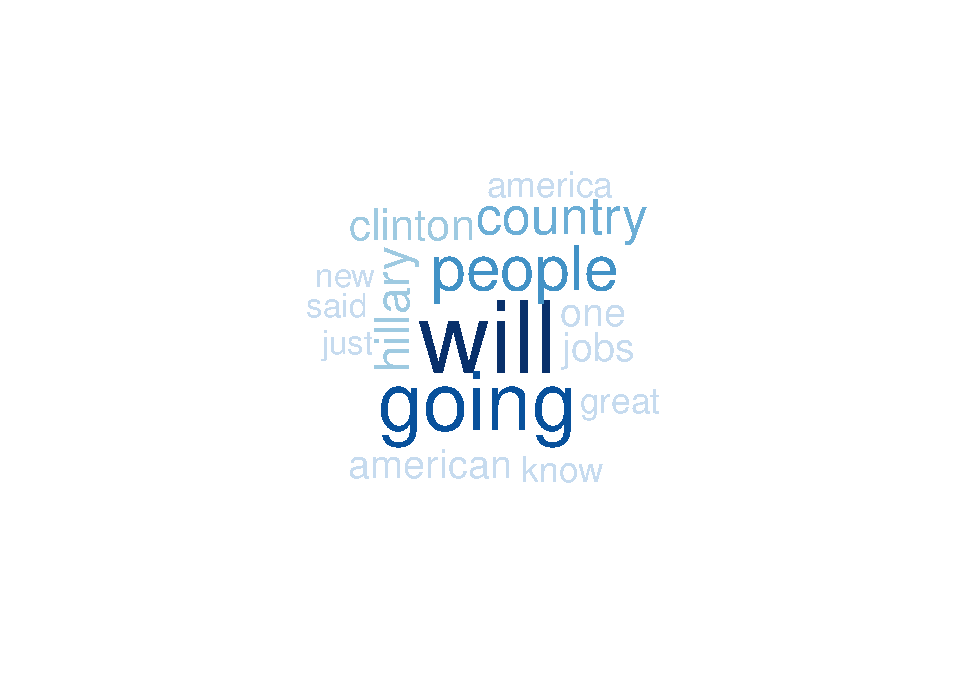
\includegraphics{Donald_Trump_Speech_sentiment_analysis_files/figure-latex/unnamed-chunk-14-1.pdf}
Now, let us get the word frequencies in a dataframe so that we can plot
them.

\begin{Shaded}
\begin{Highlighting}[]
\NormalTok{Word_freq<-}\KeywordTok{as.data.frame}\NormalTok{(Most_common)}

\KeywordTok{head}\NormalTok{(Word_freq)}
\end{Highlighting}
\end{Shaded}

\begin{verbatim}
##                 Most_common
## accomplish               51
## across                  102
## administration          191
## africanamerican         148
## ago                     120
## also                    435
\end{verbatim}

\begin{Shaded}
\begin{Highlighting}[]
\NormalTok{Word_freq}\OperatorTok{$}\NormalTok{Word<-}\KeywordTok{rownames}\NormalTok{(Word_freq)}
\KeywordTok{rownames}\NormalTok{(Word_freq)<-}\KeywordTok{c}\NormalTok{()}
\NormalTok{Word_freq<-Word_freq[}\KeywordTok{c}\NormalTok{(}\DecValTok{2}\NormalTok{,}\DecValTok{1}\NormalTok{)]}

\KeywordTok{colnames}\NormalTok{(Word_freq)<-}\KeywordTok{c}\NormalTok{(}\StringTok{"Word"}\NormalTok{,}\StringTok{"Frequency"}\NormalTok{)}
\KeywordTok{head}\NormalTok{(Word_freq)}
\end{Highlighting}
\end{Shaded}

\begin{verbatim}
##              Word Frequency
## 1      accomplish        51
## 2          across       102
## 3  administration       191
## 4 africanamerican       148
## 5             ago       120
## 6            also       435
\end{verbatim}

\begin{Shaded}
\begin{Highlighting}[]
\NormalTok{Word_freq}\OperatorTok{$}\NormalTok{Word<-}\KeywordTok{as.factor}\NormalTok{(Word_freq}\OperatorTok{$}\NormalTok{Word)}
\end{Highlighting}
\end{Shaded}

Let us now create a bar plot of the top 15 most commonly used words by
Trump.

\begin{Shaded}
\begin{Highlighting}[]
\KeywordTok{str}\NormalTok{(Word_freq)}
\end{Highlighting}
\end{Shaded}

\begin{verbatim}
## 'data.frame':    300 obs. of  2 variables:
##  $ Word     : Factor w/ 300 levels "accomplish","across",..: 1 2 3 4 5 6 7 8 9 10 ...
##  $ Frequency: num  51 102 191 148 120 435 72 91 89 632 ...
\end{verbatim}

\begin{Shaded}
\begin{Highlighting}[]
\NormalTok{Top_}\DecValTok{15}\NormalTok{<-Word_freq[}\DecValTok{1}\OperatorTok{:}\DecValTok{15}\NormalTok{,]}

\KeywordTok{dim}\NormalTok{(Top_}\DecValTok{15}\NormalTok{)}
\end{Highlighting}
\end{Shaded}

\begin{verbatim}
## [1] 15  2
\end{verbatim}

\begin{Shaded}
\begin{Highlighting}[]
\KeywordTok{ggplot}\NormalTok{(Top_}\DecValTok{15}\NormalTok{)}\OperatorTok{+}\KeywordTok{geom_bar}\NormalTok{(}\DataTypeTok{mapping =} \KeywordTok{aes}\NormalTok{(}\KeywordTok{reorder}\NormalTok{(Word,Frequency),Frequency,}\DataTypeTok{fill=}\NormalTok{Frequency),}\DataTypeTok{stat =} \StringTok{"identity"}\NormalTok{)}\OperatorTok{+}\KeywordTok{coord_flip}\NormalTok{()}
\end{Highlighting}
\end{Shaded}

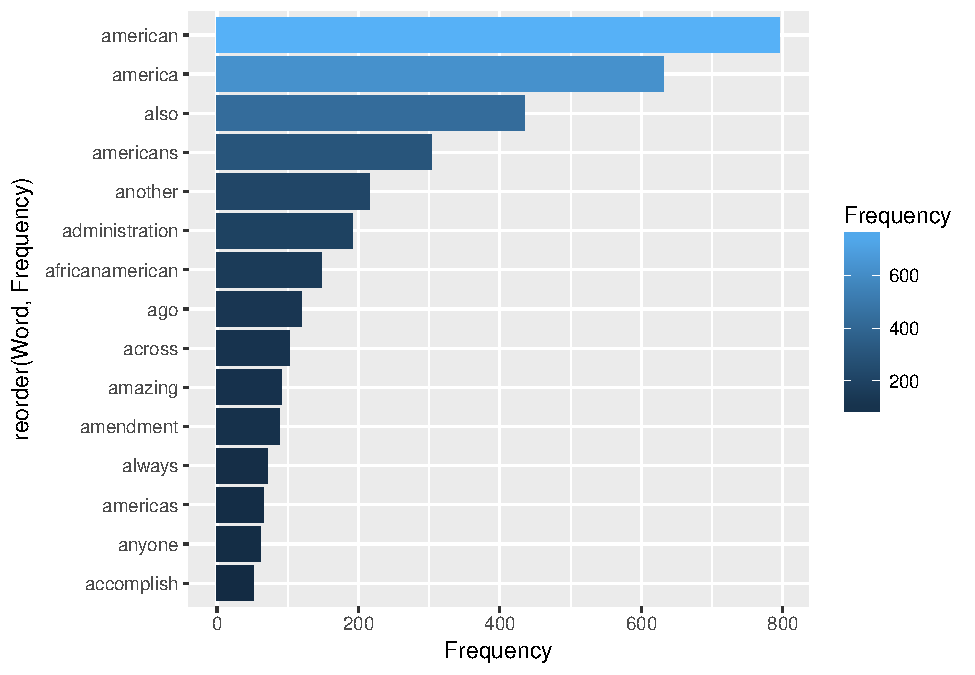
\includegraphics{Donald_Trump_Speech_sentiment_analysis_files/figure-latex/unnamed-chunk-16-1.pdf}

PART B

In this part, I will: Re-tokenize the text of all 56 Donald Trump
Speeches into a new tidy text data frame, using bigrams as tokens.
Remove each bigram where either word is a stop word or the word
``applause''. Then plot the top 15 most common bigrams in Trump's
speeches.

For the part A, I have used the corpus format. Now, I will use the
tidytext format.

\begin{Shaded}
\begin{Highlighting}[]
\NormalTok{Trump_s<-}\KeywordTok{tibble}\NormalTok{(}\DataTypeTok{line=}\DecValTok{1}\OperatorTok{:}\KeywordTok{length}\NormalTok{(Trump_speeches),}\DataTypeTok{text=}\NormalTok{Trump_speeches)}
\NormalTok{Trump_s}
\end{Highlighting}
\end{Shaded}

\begin{verbatim}
## # A tibble: 74 x 2
##     line text                                                             
##    <int> <chr>                                                            
##  1     1 "Trump: Wow. Whoa. That is some group of people. Thousands. So n~
##  2     2 " Good evening. Thank you very much. I speak to you today as a l~
##  3     3 "Thank you for the opportunity to speak to you, and thank you to~
##  4     4 "Thank you for joining me today. This was going to be a speech o~
##  5     5 "Today I'd like to share my thoughts about the stakes in this el~
##  6     6 "Thank you. I'd like to thank Chairman Jeff Miller for his leade~
##  7     7 "Thank you, everybody. Great honor. Great honor, thank you. This~
##  8     8 "Friends, delegates and fellow Americans: I humbly and gratefull~
##  9     9 "Donald Trump. So, it's been 235 days since crooked Hillary Clin~
## 10    10 "So how good is he? How good is he? [applause] Special. Special.~
## # ... with 64 more rows
\end{verbatim}

\begin{Shaded}
\begin{Highlighting}[]
\KeywordTok{dim}\NormalTok{(Trump_s)}
\end{Highlighting}
\end{Shaded}

\begin{verbatim}
## [1] 74  2
\end{verbatim}

Now, let us tidy the data.

\begin{Shaded}
\begin{Highlighting}[]
\NormalTok{tidy_speeches<-Trump_s}\OperatorTok\StringTok{ }\KeywordTok{unnest_tokens}\NormalTok{(word,text)}
\NormalTok{tidy_speeches}
\end{Highlighting}
\end{Shaded}

\begin{verbatim}
## # A tibble: 235,237 x 2
##     line word     
##    <int> <chr>    
##  1     1 trump    
##  2     1 wow      
##  3     1 whoa     
##  4     1 that     
##  5     1 is       
##  6     1 some     
##  7     1 group    
##  8     1 of       
##  9     1 people   
## 10     1 thousands
## # ... with 235,227 more rows
\end{verbatim}

Now, let us first see the most common words. This is essentially an
easier way to solve the problem 6.

Before we proceed, let us first remove the common stop words.

\begin{Shaded}
\begin{Highlighting}[]
\NormalTok{new_list<-}\KeywordTok{c}\NormalTok{(}\StringTok{"Applause"}\NormalTok{)}
\NormalTok{new_list<-}\KeywordTok{as.data.frame}\NormalTok{(new_list)}
\NormalTok{new_list}\OperatorTok{$}\NormalTok{lexicon<-}\KeywordTok{c}\NormalTok{(}\StringTok{"SMART"}\NormalTok{)}
\KeywordTok{colnames}\NormalTok{(new_list)<-}\KeywordTok{c}\NormalTok{(}\StringTok{"word"}\NormalTok{,}\StringTok{"lexicon"}\NormalTok{)}
\NormalTok{new_list}\OperatorTok{$}\NormalTok{word<-}\KeywordTok{as.character}\NormalTok{(new_list}\OperatorTok{$}\NormalTok{word)}
\NormalTok{stop_words<-}\KeywordTok{rbind}\NormalTok{(stop_words,new_list)}
\NormalTok{tidy_speeches_imp<-tidy_speeches}\OperatorTok\StringTok{ }\KeywordTok{anti_join}\NormalTok{(stop_words,}\DataTypeTok{by=}\StringTok{"word"}\NormalTok{)}\OperatorTok\StringTok{ }\KeywordTok{count}\NormalTok{(word,}\DataTypeTok{sort =} \OtherTok{TRUE}\NormalTok{)}
\end{Highlighting}
\end{Shaded}

\begin{verbatim}
## Warning: package 'bindrcpp' was built under R version 3.4.3
\end{verbatim}

\begin{Shaded}
\begin{Highlighting}[]
\NormalTok{tidy_speeches_final<-tidy_speeches_imp[}\OperatorTok{-}\DecValTok{3}\NormalTok{,] }\CommentTok{#removing the word applause}
\KeywordTok{colnames}\NormalTok{(tidy_speeches_final)<-}\KeywordTok{c}\NormalTok{(}\StringTok{"Word_used"}\NormalTok{,}\StringTok{"n"}\NormalTok{)}
\end{Highlighting}
\end{Shaded}

Now, let us plot the top 15 most used words.

\begin{Shaded}
\begin{Highlighting}[]
\NormalTok{Top15_words<-tidy_speeches_final[}\DecValTok{1}\OperatorTok{:}\DecValTok{15}\NormalTok{,]}
\KeywordTok{ggplot}\NormalTok{(Top15_words)}\OperatorTok{+}\KeywordTok{geom_bar}\NormalTok{(}\DataTypeTok{mapping =} \KeywordTok{aes}\NormalTok{(}\KeywordTok{reorder}\NormalTok{(Word_used,n),n,}\DataTypeTok{fill=}\NormalTok{n),}\DataTypeTok{stat =} \StringTok{"identity"}\NormalTok{)}\OperatorTok{+}\KeywordTok{coord_flip}\NormalTok{()}
\end{Highlighting}
\end{Shaded}

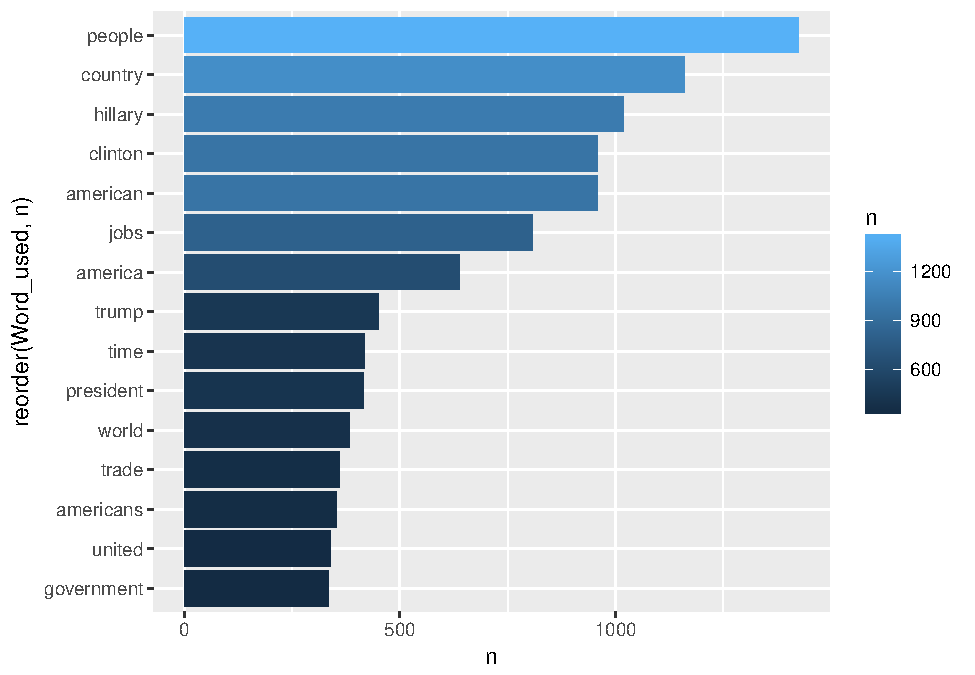
\includegraphics{Donald_Trump_Speech_sentiment_analysis_files/figure-latex/unnamed-chunk-20-1.pdf}

Now, let us create a bigram of the Trump speeches. We will do so to get
a deeper context in which the words were actually used.

\begin{Shaded}
\begin{Highlighting}[]
\NormalTok{Trump_bigrams<-Trump_s}\OperatorTok\StringTok{ }\KeywordTok{unnest_tokens}\NormalTok{(bigram,text,}\DataTypeTok{token =} \StringTok{"ngrams"}\NormalTok{,}\DataTypeTok{n=}\DecValTok{2}\NormalTok{)}
\NormalTok{Trump_bigrams}
\end{Highlighting}
\end{Shaded}

\begin{verbatim}
## # A tibble: 235,163 x 2
##     line bigram          
##    <int> <chr>           
##  1     1 trump wow       
##  2     1 wow whoa        
##  3     1 whoa that       
##  4     1 that is         
##  5     1 is some         
##  6     1 some group      
##  7     1 group of        
##  8     1 of people       
##  9     1 people thousands
## 10     1 thousands so    
## # ... with 235,153 more rows
\end{verbatim}

\begin{Shaded}
\begin{Highlighting}[]
\NormalTok{tidy_speeches_big<-tidy_speeches}\OperatorTok\StringTok{ }\KeywordTok{anti_join}\NormalTok{(stop_words,}\DataTypeTok{by=}\StringTok{"word"}\NormalTok{)}
\KeywordTok{str}\NormalTok{(tidy_speeches_big)}
\end{Highlighting}
\end{Shaded}

\begin{verbatim}
## Classes 'tbl_df', 'tbl' and 'data.frame':    85814 obs. of  2 variables:
##  $ line: int  1 1 1 1 1 1 1 1 1 1 ...
##  $ word: chr  "trump" "wow" "whoa" "people" ...
\end{verbatim}

\begin{Shaded}
\begin{Highlighting}[]
\KeywordTok{str}\NormalTok{(Trump_s)}
\end{Highlighting}
\end{Shaded}

\begin{verbatim}
## Classes 'tbl_df', 'tbl' and 'data.frame':    74 obs. of  2 variables:
##  $ line: int  1 2 3 4 5 6 7 8 9 10 ...
##  $ text: chr  "Trump: Wow. Whoa. That is some group of people. Thousands. So nice, thank you very much. That's really nice. Th"| __truncated__ " Good evening. Thank you very much. I speak to you today as a lifelong supporter and true friend of Israel. I'm"| __truncated__ "Thank you for the opportunity to speak to you, and thank you to the Center for the National Interest for honori"| __truncated__ "Thank you for joining me today. This was going to be a speech on Hillary Clinton and how bad a President, espec"| __truncated__ ...
\end{verbatim}

Now let us check the most common bigrams.

\begin{Shaded}
\begin{Highlighting}[]
\NormalTok{Trump_bigrams<-Trump_bigrams}\OperatorTok\KeywordTok{count}\NormalTok{(bigram,}\DataTypeTok{sort =} \OtherTok{TRUE}\NormalTok{)}
\NormalTok{Trump_bigrams}
\end{Highlighting}
\end{Shaded}

\begin{verbatim}
## # A tibble: 76,867 x 2
##    bigram              n
##    <chr>           <int>
##  1 going to         1821
##  2 of the            987
##  3 we will           819
##  4 we are            710
##  5 in the            669
##  6 hillary clinton   663
##  7 our country       575
##  8 are going         558
##  9 to be             538
## 10 we have           473
## # ... with 76,857 more rows
\end{verbatim}

We can see that there are still stop words in the bigrams which we
should eliminate.

For that, we will first split the bigrams into two words, eliminate the
stop words and then reunite the words to form a bigram again.

\begin{Shaded}
\begin{Highlighting}[]
\KeywordTok{library}\NormalTok{(tidyr)}
\NormalTok{Trump_bigrams_sep<-Trump_bigrams}\OperatorTok\KeywordTok{separate}\NormalTok{(bigram,}\KeywordTok{c}\NormalTok{(}\StringTok{"word1"}\NormalTok{,}\StringTok{"word2"}\NormalTok{),}\DataTypeTok{sep =} \StringTok{" "}\NormalTok{)}
\NormalTok{Trump_bigrams_sep}
\end{Highlighting}
\end{Shaded}

\begin{verbatim}
## # A tibble: 76,867 x 3
##    word1   word2       n
##  * <chr>   <chr>   <int>
##  1 going   to       1821
##  2 of      the       987
##  3 we      will      819
##  4 we      are       710
##  5 in      the       669
##  6 hillary clinton   663
##  7 our     country   575
##  8 are     going     558
##  9 to      be        538
## 10 we      have      473
## # ... with 76,857 more rows
\end{verbatim}

\begin{Shaded}
\begin{Highlighting}[]
\NormalTok{Trump_bigrams_sep<-Trump_bigrams_sep}\OperatorTok\StringTok{ }\KeywordTok{filter}\NormalTok{(}\OperatorTok{!}\NormalTok{word1 }\OperatorTok\StringTok{ }\NormalTok{stop_words}\OperatorTok{$}\NormalTok{word)}\OperatorTok\KeywordTok{filter}\NormalTok{(}\OperatorTok{!}\NormalTok{word2 }\OperatorTok\StringTok{ }\NormalTok{stop_words}\OperatorTok{$}\NormalTok{word)}

\NormalTok{Trump_bigrams_sep}
\end{Highlighting}
\end{Shaded}

\begin{verbatim}
## # A tibble: 14,257 x 3
##    word1     word2              n
##    <chr>     <chr>          <int>
##  1 hillary   clinton          663
##  2 donald    trump            172
##  3 african   american         164
##  4 american  people           119
##  5 trump     administration   112
##  6 hillary   clinton's        104
##  7 trade     deals            102
##  8 november  8th               91
##  9 middle    east              88
## 10 president obama             87
## # ... with 14,247 more rows
\end{verbatim}

Now let us unite these bigrams again so that we can plot it.

\begin{Shaded}
\begin{Highlighting}[]
\NormalTok{Trump_bigrams_final<-Trump_bigrams_sep}\OperatorTok\StringTok{ }\KeywordTok{unite}\NormalTok{(bigram,word1,word2,}\DataTypeTok{sep =} \StringTok{" "}\NormalTok{)}
\NormalTok{Trump_bigrams_final}
\end{Highlighting}
\end{Shaded}

\begin{verbatim}
## # A tibble: 14,257 x 2
##    bigram                   n
##  * <chr>                <int>
##  1 hillary clinton        663
##  2 donald trump           172
##  3 african american       164
##  4 american people        119
##  5 trump administration   112
##  6 hillary clinton's      104
##  7 trade deals            102
##  8 november 8th            91
##  9 middle east             88
## 10 president obama         87
## # ... with 14,247 more rows
\end{verbatim}

Now, let us plot the top 15 most commonly used bigrams in Trump's
speeches.

\begin{Shaded}
\begin{Highlighting}[]
\NormalTok{Top15_bigram<-Trump_bigrams_final[}\DecValTok{1}\OperatorTok{:}\DecValTok{15}\NormalTok{,]}
\KeywordTok{ggplot}\NormalTok{(Top15_bigram)}\OperatorTok{+}\KeywordTok{geom_bar}\NormalTok{(}\DataTypeTok{mapping =} \KeywordTok{aes}\NormalTok{(}\KeywordTok{reorder}\NormalTok{(bigram,n),n,}\DataTypeTok{fill=}\NormalTok{n),}\DataTypeTok{stat =} \StringTok{"identity"}\NormalTok{)}\OperatorTok{+}\KeywordTok{coord_flip}\NormalTok{()}
\end{Highlighting}
\end{Shaded}

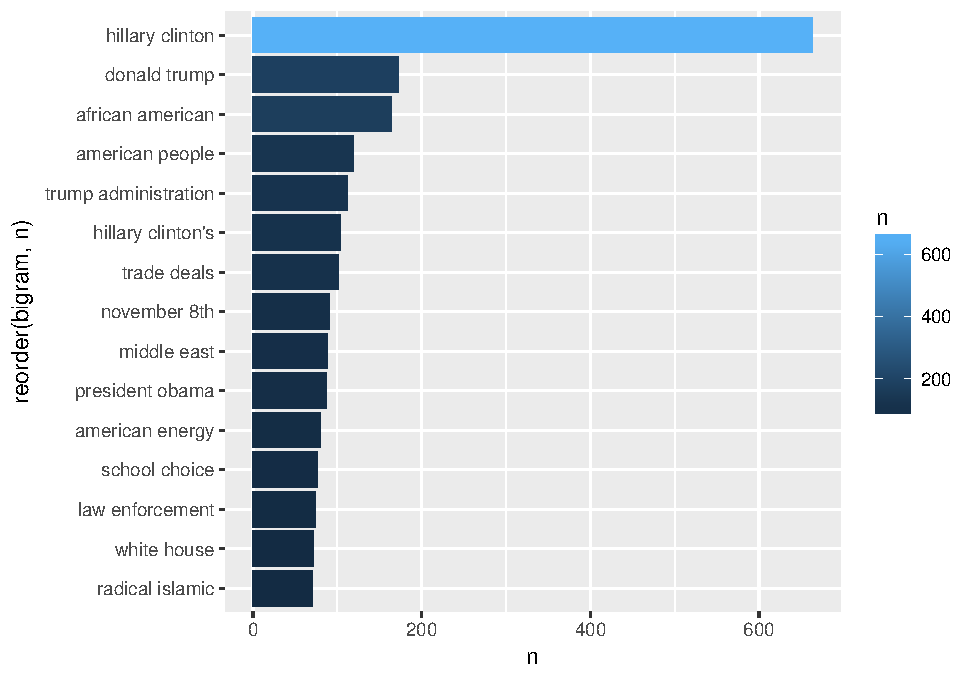
\includegraphics{Donald_Trump_Speech_sentiment_analysis_files/figure-latex/unnamed-chunk-26-1.pdf}

PART C

For the part C, I will do the following:

A sentiment analysis of Donald Trump's speeches. In order to make sure
sentiments are assigned to appropriate contexts, first tokenize the
speeches into bigrams, and then filter out all bigrams where the first
word is any of ``not'', ``no'', or ``never''.

Now, we have to remove the bigrams where the first words are
``no'',``not'',``never''.

For that, let us use the separated bigrams from the previous question.

\begin{Shaded}
\begin{Highlighting}[]
\NormalTok{Negative<-}\KeywordTok{c}\NormalTok{(}\StringTok{"no"}\NormalTok{,}\StringTok{"not"}\NormalTok{,}\StringTok{"never"}\NormalTok{)}
\NormalTok{Tr<-}\KeywordTok{c}\NormalTok{(}\StringTok{"trump"}\NormalTok{,}\StringTok{"applause"}\NormalTok{)}
\NormalTok{Trump_bigram_senti<-Trump_bigrams_sep}\OperatorTok\StringTok{ }\KeywordTok{filter}\NormalTok{(}\OperatorTok{!}\NormalTok{word1 }\OperatorTok\StringTok{ }\NormalTok{Negative)}\OperatorTok\StringTok{ }\KeywordTok{filter}\NormalTok{(}\OperatorTok{!}\NormalTok{word2}\OperatorTok\StringTok{ }\NormalTok{Tr)}

\NormalTok{Trump_bigram_senti}\OperatorTok\StringTok{ }\KeywordTok{filter}\NormalTok{(word2}\OperatorTok{==}\StringTok{"trump"}\NormalTok{)}\CommentTok{# checking if the word elimination worked.}
\end{Highlighting}
\end{Shaded}

\begin{verbatim}
## # A tibble: 0 x 3
## # ... with 3 variables: word1 <chr>, word2 <chr>, n <int>
\end{verbatim}

\begin{Shaded}
\begin{Highlighting}[]
\NormalTok{Trump_bigram_senti}\OperatorTok\StringTok{ }\KeywordTok{filter}\NormalTok{(word1}\OperatorTok{==}\StringTok{"no"}\NormalTok{)}
\end{Highlighting}
\end{Shaded}

\begin{verbatim}
## # A tibble: 0 x 3
## # ... with 3 variables: word1 <chr>, word2 <chr>, n <int>
\end{verbatim}

Now let us get each of the 10 sentiments in the nrc into 10 separate
dataframes.

We will need these to do the further analysis.

\begin{Shaded}
\begin{Highlighting}[]
\NormalTok{nrc<-}\KeywordTok{get_sentiments}\NormalTok{(}\StringTok{"nrc"}\NormalTok{)}
\KeywordTok{unique}\NormalTok{(nrc}\OperatorTok{$}\NormalTok{sentiment)}
\end{Highlighting}
\end{Shaded}

\begin{verbatim}
##  [1] "trust"        "fear"         "negative"     "sadness"     
##  [5] "anger"        "surprise"     "positive"     "disgust"     
##  [9] "joy"          "anticipation"
\end{verbatim}

\begin{Shaded}
\begin{Highlighting}[]
\NormalTok{nrc_trust<-nrc}\OperatorTok\KeywordTok{filter}\NormalTok{(sentiment}\OperatorTok{==}\StringTok{"trust"}\NormalTok{)}
\NormalTok{nrc_fear<-nrc}\OperatorTok\KeywordTok{filter}\NormalTok{(sentiment}\OperatorTok{==}\StringTok{"fear"}\NormalTok{)}
\NormalTok{nrc_negative<-nrc}\OperatorTok\KeywordTok{filter}\NormalTok{(sentiment}\OperatorTok{==}\StringTok{"negative"}\NormalTok{)}
\NormalTok{nrc_sadness<-nrc}\OperatorTok\KeywordTok{filter}\NormalTok{(sentiment}\OperatorTok{==}\StringTok{"sadness"}\NormalTok{)}
\NormalTok{nrc_anger<-nrc}\OperatorTok\KeywordTok{filter}\NormalTok{(sentiment}\OperatorTok{==}\StringTok{"anger"}\NormalTok{)}
\NormalTok{nrc_surprise<-nrc}\OperatorTok\KeywordTok{filter}\NormalTok{(sentiment}\OperatorTok{==}\StringTok{"suprise"}\NormalTok{)}
\NormalTok{nrc_positive<-nrc}\OperatorTok\KeywordTok{filter}\NormalTok{(sentiment}\OperatorTok{==}\StringTok{"positive"}\NormalTok{)}
\NormalTok{nrc_disgust<-nrc}\OperatorTok\KeywordTok{filter}\NormalTok{(sentiment}\OperatorTok{==}\StringTok{"disgust"}\NormalTok{)}
\NormalTok{nrc_joy<-nrc}\OperatorTok\KeywordTok{filter}\NormalTok{(sentiment}\OperatorTok{==}\StringTok{"joy"}\NormalTok{)}
\NormalTok{nrc_anticipation<-nrc}\OperatorTok\KeywordTok{filter}\NormalTok{(sentiment}\OperatorTok{==}\StringTok{"anticipation"}\NormalTok{)}
\end{Highlighting}
\end{Shaded}

Let us first create a new column in our dataframe so that we can later
join the sentiment dataframes.

\begin{Shaded}
\begin{Highlighting}[]
\NormalTok{Trump_bigram_senti}\OperatorTok{$}\NormalTok{word<-Trump_bigram_senti}\OperatorTok{$}\NormalTok{word2}
\NormalTok{Trump_sentiment<-Trump_bigram_senti[,}\DecValTok{4}\NormalTok{]}
\KeywordTok{class}\NormalTok{(Trump_sentiment)}
\end{Highlighting}
\end{Shaded}

\begin{verbatim}
## [1] "tbl_df"     "tbl"        "data.frame"
\end{verbatim}

Now, let us see the top 10 words in Trump's speeches associated with
trust.

\begin{Shaded}
\begin{Highlighting}[]
\NormalTok{Trust_trump<-Trump_sentiment}\OperatorTok\StringTok{ }\KeywordTok{inner_join}\NormalTok{(nrc_trust,}\DataTypeTok{by=}\StringTok{"word"}\NormalTok{)}\OperatorTok\StringTok{ }\KeywordTok{count}\NormalTok{(word)}\OperatorTok\KeywordTok{top_n}\NormalTok{(}\DecValTok{10}\NormalTok{)}
\end{Highlighting}
\end{Shaded}

\begin{verbatim}
## Selecting by n
\end{verbatim}

\begin{Shaded}
\begin{Highlighting}[]
\KeywordTok{ggplot}\NormalTok{(Trust_trump)}\OperatorTok{+}\KeywordTok{geom_bar}\NormalTok{(}\DataTypeTok{mapping =} \KeywordTok{aes}\NormalTok{(}\KeywordTok{reorder}\NormalTok{(word,n),n,}\DataTypeTok{fill=}\NormalTok{n),}\DataTypeTok{stat =} \StringTok{"identity"}\NormalTok{)}\OperatorTok{+}\KeywordTok{coord_flip}\NormalTok{()}\OperatorTok{+}\KeywordTok{labs}\NormalTok{(}\DataTypeTok{x=}\StringTok{"Trust_words"}\NormalTok{,}\DataTypeTok{y=}\StringTok{"Number"}\NormalTok{)}
\end{Highlighting}
\end{Shaded}

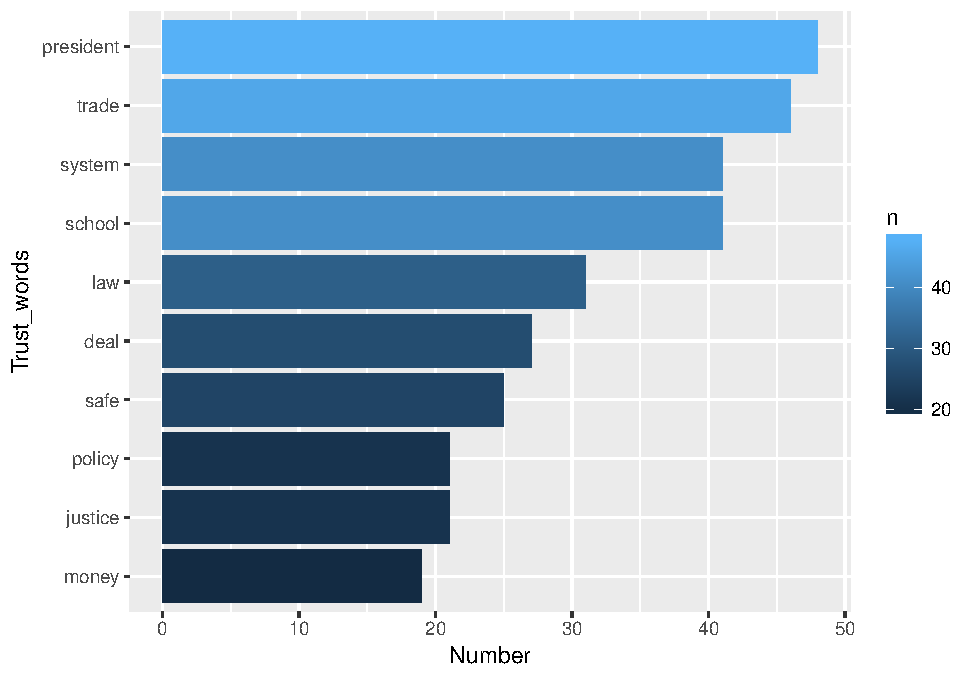
\includegraphics{Donald_Trump_Speech_sentiment_analysis_files/figure-latex/unnamed-chunk-30-1.pdf}
Now, let us see the top 10 words in Trump's speeches associated with
Fear.

\begin{Shaded}
\begin{Highlighting}[]
\NormalTok{Fear_trump<-Trump_sentiment}\OperatorTok\StringTok{ }\KeywordTok{inner_join}\NormalTok{(nrc_fear,}\DataTypeTok{by=}\StringTok{"word"}\NormalTok{)}\OperatorTok\StringTok{ }\KeywordTok{count}\NormalTok{(word)}\OperatorTok\KeywordTok{top_n}\NormalTok{(}\DecValTok{10}\NormalTok{)}
\end{Highlighting}
\end{Shaded}

\begin{verbatim}
## Selecting by n
\end{verbatim}

\begin{Shaded}
\begin{Highlighting}[]
\KeywordTok{ggplot}\NormalTok{(Fear_trump)}\OperatorTok{+}\KeywordTok{geom_bar}\NormalTok{(}\DataTypeTok{mapping =} \KeywordTok{aes}\NormalTok{(}\KeywordTok{reorder}\NormalTok{(word,n),n,}\DataTypeTok{fill=}\NormalTok{n),}\DataTypeTok{stat =} \StringTok{"identity"}\NormalTok{)}\OperatorTok{+}\KeywordTok{coord_flip}\NormalTok{()}\OperatorTok{+}\KeywordTok{labs}\NormalTok{(}\DataTypeTok{x=}\StringTok{"Fear_words"}\NormalTok{,}\DataTypeTok{y=}\StringTok{"Number"}\NormalTok{)}
\end{Highlighting}
\end{Shaded}

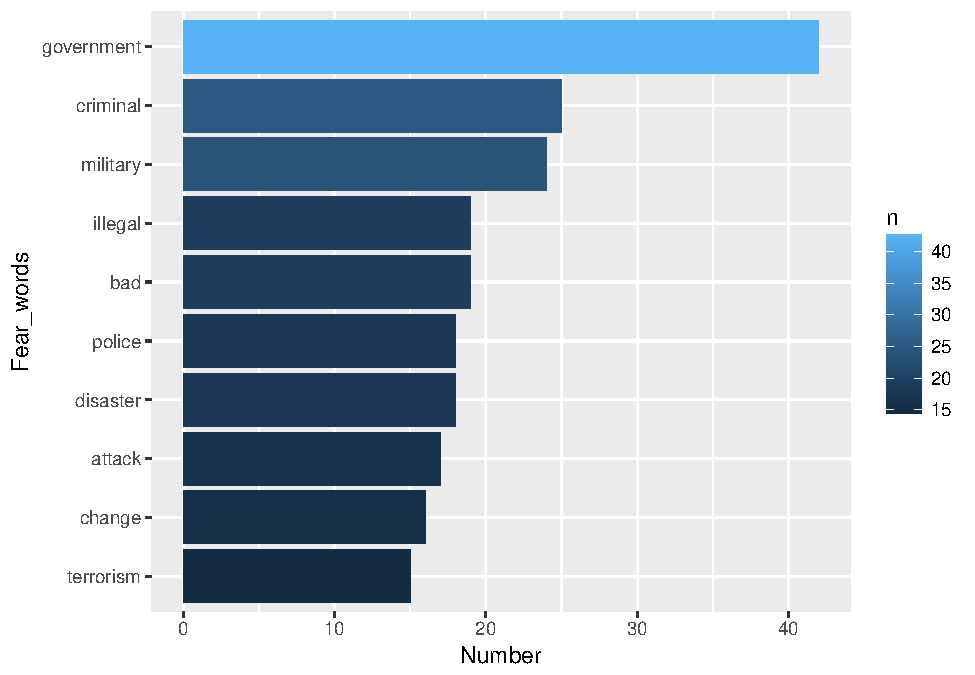
\includegraphics{Donald_Trump_Speech_sentiment_analysis_files/figure-latex/unnamed-chunk-31-1.pdf}

Now, let us see the top 10 words in Trump's speeches associated with
negative.

\begin{Shaded}
\begin{Highlighting}[]
\NormalTok{Negative_trump<-Trump_sentiment}\OperatorTok\StringTok{ }\KeywordTok{inner_join}\NormalTok{(nrc_negative,}\DataTypeTok{by=}\StringTok{"word"}\NormalTok{)}\OperatorTok\StringTok{ }\KeywordTok{count}\NormalTok{(word)}\OperatorTok\KeywordTok{top_n}\NormalTok{(}\DecValTok{10}\NormalTok{)}
\end{Highlighting}
\end{Shaded}

\begin{verbatim}
## Selecting by n
\end{verbatim}

\begin{Shaded}
\begin{Highlighting}[]
\KeywordTok{ggplot}\NormalTok{(Negative_trump)}\OperatorTok{+}\KeywordTok{geom_bar}\NormalTok{(}\DataTypeTok{mapping =} \KeywordTok{aes}\NormalTok{(}\KeywordTok{reorder}\NormalTok{(word,n),n,}\DataTypeTok{fill=}\NormalTok{n),}\DataTypeTok{stat =} \StringTok{"identity"}\NormalTok{)}\OperatorTok{+}\KeywordTok{coord_flip}\NormalTok{()}\OperatorTok{+}\KeywordTok{labs}\NormalTok{(}\DataTypeTok{x=}\StringTok{"Negative_words"}\NormalTok{,}\DataTypeTok{y=}\StringTok{"Number"}\NormalTok{)}
\end{Highlighting}
\end{Shaded}

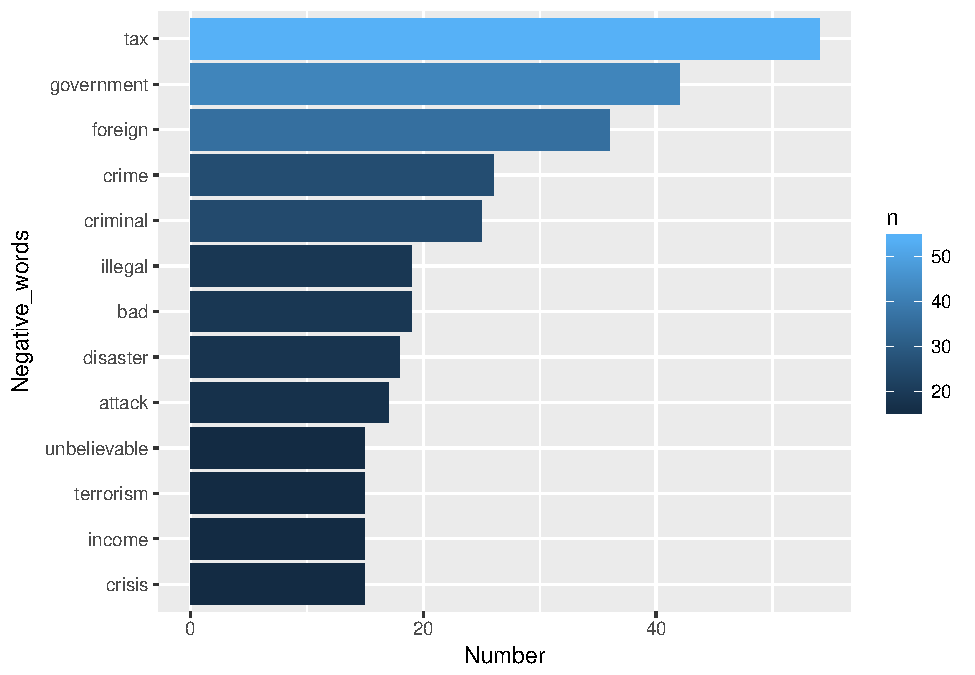
\includegraphics{Donald_Trump_Speech_sentiment_analysis_files/figure-latex/unnamed-chunk-32-1.pdf}

Now, let us see the top 10 words in Trump's speeches associated with
sadness.

\begin{Shaded}
\begin{Highlighting}[]
\NormalTok{Sad_trump<-Trump_sentiment}\OperatorTok\StringTok{ }\KeywordTok{inner_join}\NormalTok{(nrc_sadness,}\DataTypeTok{by=}\StringTok{"word"}\NormalTok{)}\OperatorTok\StringTok{ }\KeywordTok{count}\NormalTok{(word)}\OperatorTok\KeywordTok{top_n}\NormalTok{(}\DecValTok{10}\NormalTok{)}
\end{Highlighting}
\end{Shaded}

\begin{verbatim}
## Selecting by n
\end{verbatim}

\begin{Shaded}
\begin{Highlighting}[]
\KeywordTok{ggplot}\NormalTok{(Sad_trump)}\OperatorTok{+}\KeywordTok{geom_bar}\NormalTok{(}\DataTypeTok{mapping =} \KeywordTok{aes}\NormalTok{(}\KeywordTok{reorder}\NormalTok{(word,n),n,}\DataTypeTok{fill=}\NormalTok{n),}\DataTypeTok{stat =} \StringTok{"identity"}\NormalTok{)}\OperatorTok{+}\KeywordTok{coord_flip}\NormalTok{()}\OperatorTok{+}\KeywordTok{labs}\NormalTok{(}\DataTypeTok{x=}\StringTok{"Sad_words"}\NormalTok{,}\DataTypeTok{y=}\StringTok{"Number"}\NormalTok{)}
\end{Highlighting}
\end{Shaded}

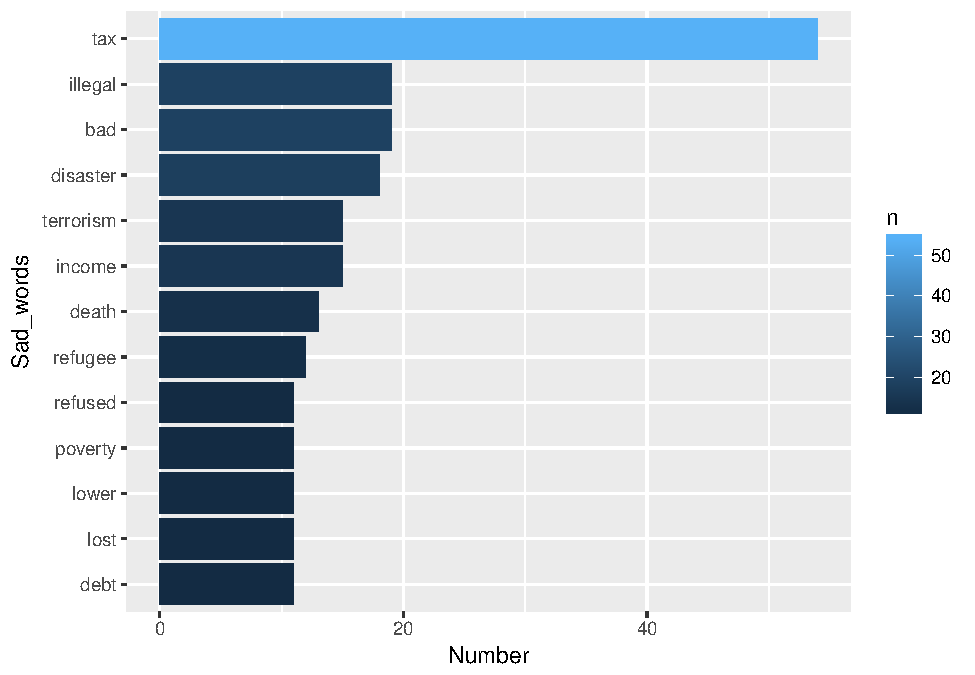
\includegraphics{Donald_Trump_Speech_sentiment_analysis_files/figure-latex/unnamed-chunk-33-1.pdf}

Now, let us see the top 10 words in Trump's speeches associated with
anger.

\begin{Shaded}
\begin{Highlighting}[]
\NormalTok{Anger_trump<-Trump_sentiment}\OperatorTok\StringTok{ }\KeywordTok{inner_join}\NormalTok{(nrc_anger,}\DataTypeTok{by=}\StringTok{"word"}\NormalTok{)}\OperatorTok\StringTok{ }\KeywordTok{count}\NormalTok{(word)}\OperatorTok\KeywordTok{top_n}\NormalTok{(}\DecValTok{10}\NormalTok{)}
\end{Highlighting}
\end{Shaded}

\begin{verbatim}
## Selecting by n
\end{verbatim}

\begin{Shaded}
\begin{Highlighting}[]
\KeywordTok{ggplot}\NormalTok{(Anger_trump)}\OperatorTok{+}\KeywordTok{geom_bar}\NormalTok{(}\DataTypeTok{mapping =} \KeywordTok{aes}\NormalTok{(}\KeywordTok{reorder}\NormalTok{(word,n),n,}\DataTypeTok{fill=}\NormalTok{n),}\DataTypeTok{stat =} \StringTok{"identity"}\NormalTok{)}\OperatorTok{+}\KeywordTok{coord_flip}\NormalTok{()}\OperatorTok{+}\KeywordTok{labs}\NormalTok{(}\DataTypeTok{x=}\StringTok{"Anger_words"}\NormalTok{,}\DataTypeTok{y=}\StringTok{"Number"}\NormalTok{)}
\end{Highlighting}
\end{Shaded}

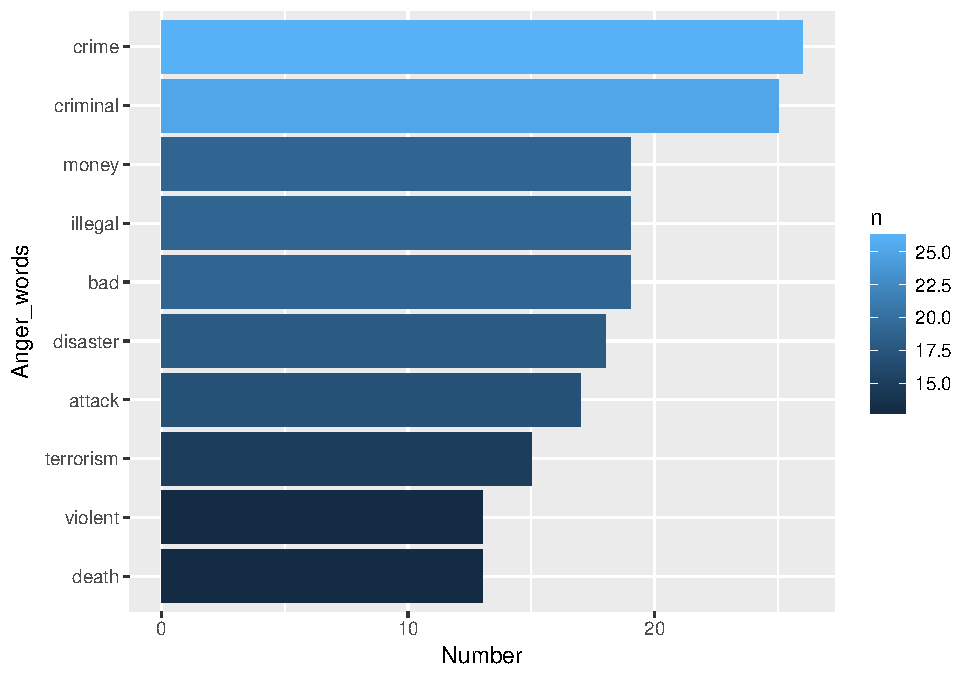
\includegraphics{Donald_Trump_Speech_sentiment_analysis_files/figure-latex/unnamed-chunk-34-1.pdf}

Now, let us see the top 10 words in Trump's speeches associated with
surprise.

\begin{Shaded}
\begin{Highlighting}[]
\NormalTok{Surprise_trump<-Trump_sentiment}\OperatorTok\StringTok{ }\KeywordTok{inner_join}\NormalTok{(nrc_surprise,}\DataTypeTok{by=}\StringTok{"word"}\NormalTok{)}\OperatorTok\StringTok{ }\KeywordTok{count}\NormalTok{(word)}\OperatorTok\KeywordTok{top_n}\NormalTok{(}\DecValTok{10}\NormalTok{)}
\end{Highlighting}
\end{Shaded}

\begin{verbatim}
## Selecting by n
\end{verbatim}

\begin{Shaded}
\begin{Highlighting}[]
\KeywordTok{ggplot}\NormalTok{(Surprise_trump)}\OperatorTok{+}\KeywordTok{geom_bar}\NormalTok{(}\DataTypeTok{mapping =} \KeywordTok{aes}\NormalTok{(}\KeywordTok{reorder}\NormalTok{(word,n),n,}\DataTypeTok{fill=}\NormalTok{n),}\DataTypeTok{stat =} \StringTok{"identity"}\NormalTok{)}\OperatorTok{+}\KeywordTok{coord_flip}\NormalTok{()}\OperatorTok{+}\KeywordTok{labs}\NormalTok{(}\DataTypeTok{x=}\StringTok{"Trust_words"}\NormalTok{,}\DataTypeTok{y=}\StringTok{"Number"}\NormalTok{)}
\end{Highlighting}
\end{Shaded}

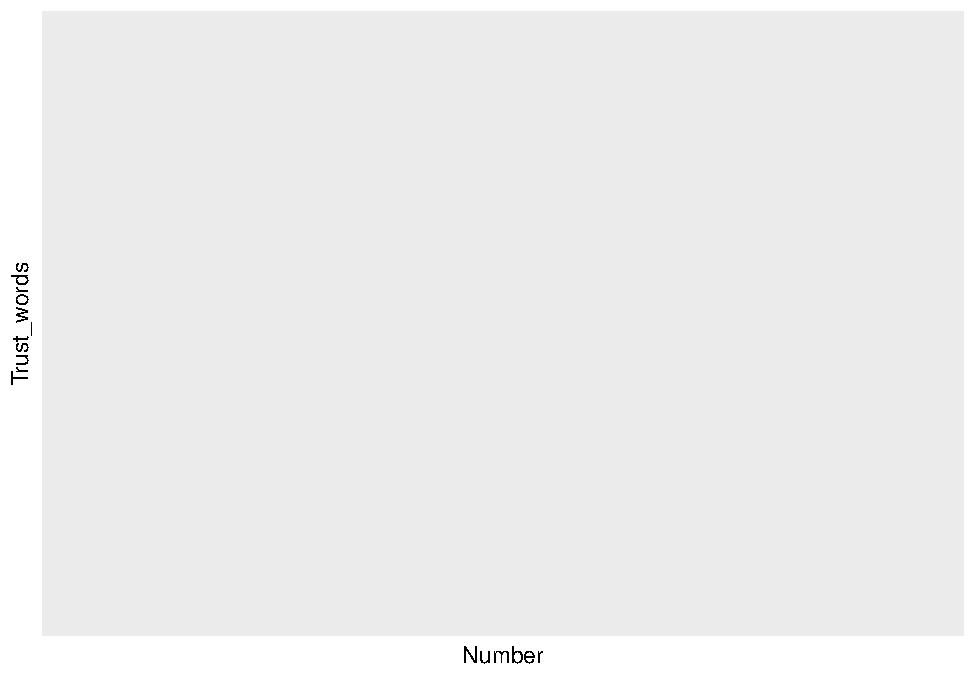
\includegraphics{Donald_Trump_Speech_sentiment_analysis_files/figure-latex/unnamed-chunk-35-1.pdf}
There are no surprise words in trump's speeches.

Now, let us see the top 10 words in Trump's speeches associated with
positive.

\begin{Shaded}
\begin{Highlighting}[]
\NormalTok{Positive_trump<-Trump_sentiment}\OperatorTok\StringTok{ }\KeywordTok{inner_join}\NormalTok{(nrc_positive,}\DataTypeTok{by=}\StringTok{"word"}\NormalTok{)}\OperatorTok\StringTok{ }\KeywordTok{count}\NormalTok{(word)}\OperatorTok\KeywordTok{top_n}\NormalTok{(}\DecValTok{10}\NormalTok{)}
\end{Highlighting}
\end{Shaded}

\begin{verbatim}
## Selecting by n
\end{verbatim}

\begin{Shaded}
\begin{Highlighting}[]
\KeywordTok{ggplot}\NormalTok{(Positive_trump)}\OperatorTok{+}\KeywordTok{geom_bar}\NormalTok{(}\DataTypeTok{mapping =} \KeywordTok{aes}\NormalTok{(}\KeywordTok{reorder}\NormalTok{(word,n),n,}\DataTypeTok{fill=}\NormalTok{n),}\DataTypeTok{stat =} \StringTok{"identity"}\NormalTok{)}\OperatorTok{+}\KeywordTok{coord_flip}\NormalTok{()}\OperatorTok{+}\KeywordTok{labs}\NormalTok{(}\DataTypeTok{x=}\StringTok{"Positive_words"}\NormalTok{,}\DataTypeTok{y=}\StringTok{"Number"}\NormalTok{)}
\end{Highlighting}
\end{Shaded}

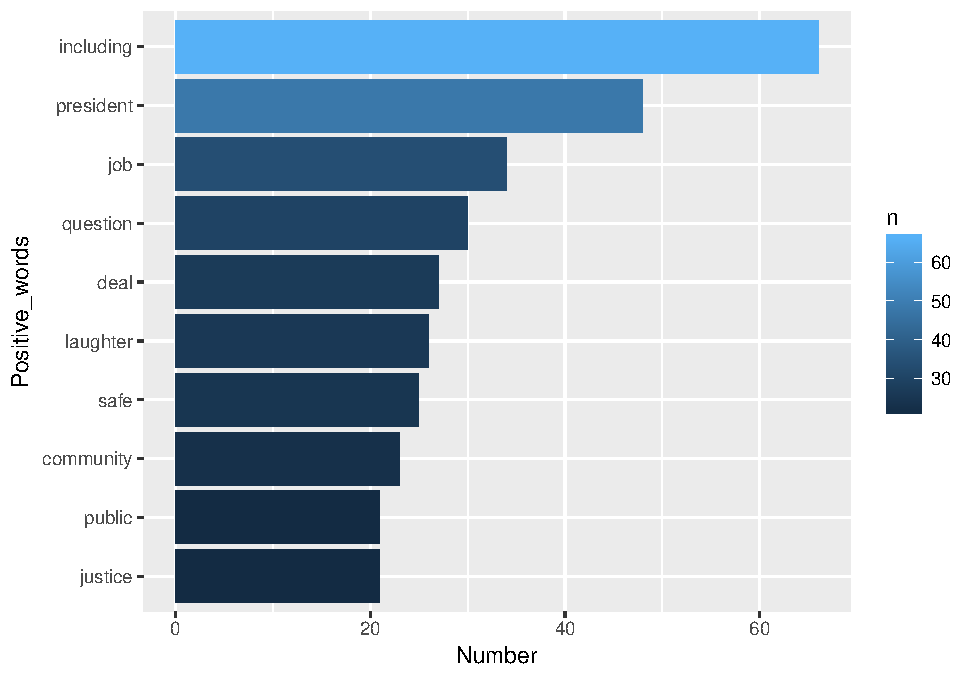
\includegraphics{Donald_Trump_Speech_sentiment_analysis_files/figure-latex/unnamed-chunk-36-1.pdf}

Now, let us see the top 10 words in Trump's speeches associated with
disgust.

\begin{Shaded}
\begin{Highlighting}[]
\NormalTok{disgust_trump<-Trump_sentiment}\OperatorTok\StringTok{ }\KeywordTok{inner_join}\NormalTok{(nrc_disgust,}\DataTypeTok{by=}\StringTok{"word"}\NormalTok{)}\OperatorTok\StringTok{ }\KeywordTok{count}\NormalTok{(word)}\OperatorTok\KeywordTok{top_n}\NormalTok{(}\DecValTok{10}\NormalTok{)}
\end{Highlighting}
\end{Shaded}

\begin{verbatim}
## Selecting by n
\end{verbatim}

\begin{Shaded}
\begin{Highlighting}[]
\KeywordTok{ggplot}\NormalTok{(disgust_trump)}\OperatorTok{+}\KeywordTok{geom_bar}\NormalTok{(}\DataTypeTok{mapping =} \KeywordTok{aes}\NormalTok{(}\KeywordTok{reorder}\NormalTok{(word,n),n,}\DataTypeTok{fill=}\NormalTok{n),}\DataTypeTok{stat =} \StringTok{"identity"}\NormalTok{)}\OperatorTok{+}\KeywordTok{coord_flip}\NormalTok{()}\OperatorTok{+}\KeywordTok{labs}\NormalTok{(}\DataTypeTok{x=}\StringTok{"Disgust_words"}\NormalTok{,}\DataTypeTok{y=}\StringTok{"Number"}\NormalTok{)}
\end{Highlighting}
\end{Shaded}

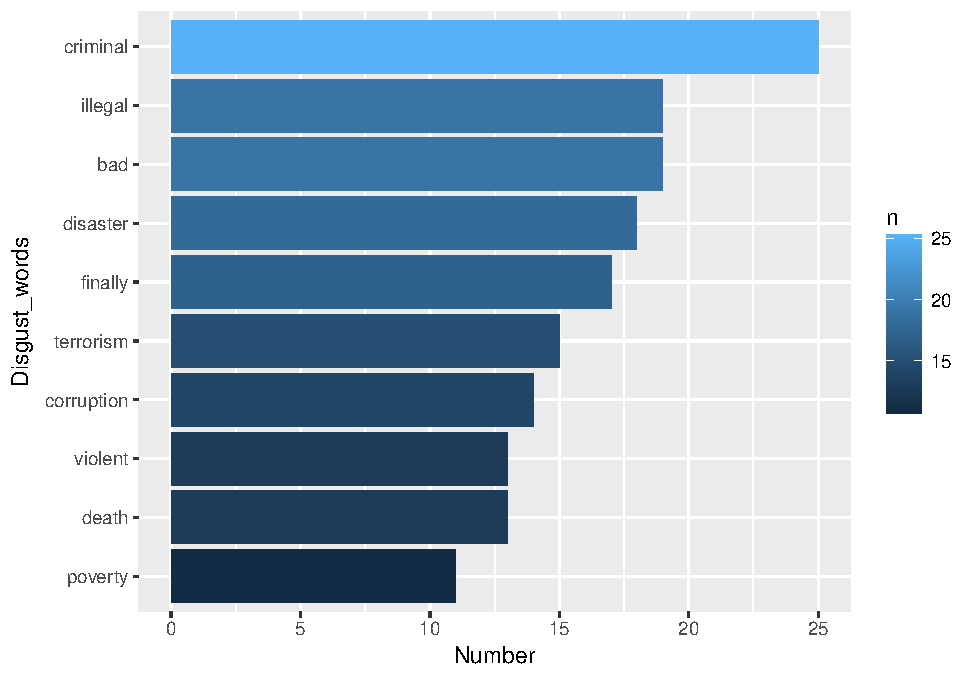
\includegraphics{Donald_Trump_Speech_sentiment_analysis_files/figure-latex/unnamed-chunk-37-1.pdf}

Now, let us see the top 10 words in Trump's speeches associated with
joy.

\begin{Shaded}
\begin{Highlighting}[]
\NormalTok{joy_trump<-Trump_sentiment}\OperatorTok\StringTok{ }\KeywordTok{inner_join}\NormalTok{(nrc_joy,}\DataTypeTok{by=}\StringTok{"word"}\NormalTok{)}\OperatorTok\StringTok{ }\KeywordTok{count}\NormalTok{(word)}\OperatorTok\KeywordTok{top_n}\NormalTok{(}\DecValTok{10}\NormalTok{)}
\end{Highlighting}
\end{Shaded}

\begin{verbatim}
## Selecting by n
\end{verbatim}

\begin{Shaded}
\begin{Highlighting}[]
\KeywordTok{ggplot}\NormalTok{(joy_trump)}\OperatorTok{+}\KeywordTok{geom_bar}\NormalTok{(}\DataTypeTok{mapping =} \KeywordTok{aes}\NormalTok{(}\KeywordTok{reorder}\NormalTok{(word,n),n,}\DataTypeTok{fill=}\NormalTok{n),}\DataTypeTok{stat =} \StringTok{"identity"}\NormalTok{)}\OperatorTok{+}\KeywordTok{coord_flip}\NormalTok{()}\OperatorTok{+}\KeywordTok{labs}\NormalTok{(}\DataTypeTok{x=}\StringTok{"Joy_words"}\NormalTok{,}\DataTypeTok{y=}\StringTok{"Number"}\NormalTok{)}
\end{Highlighting}
\end{Shaded}

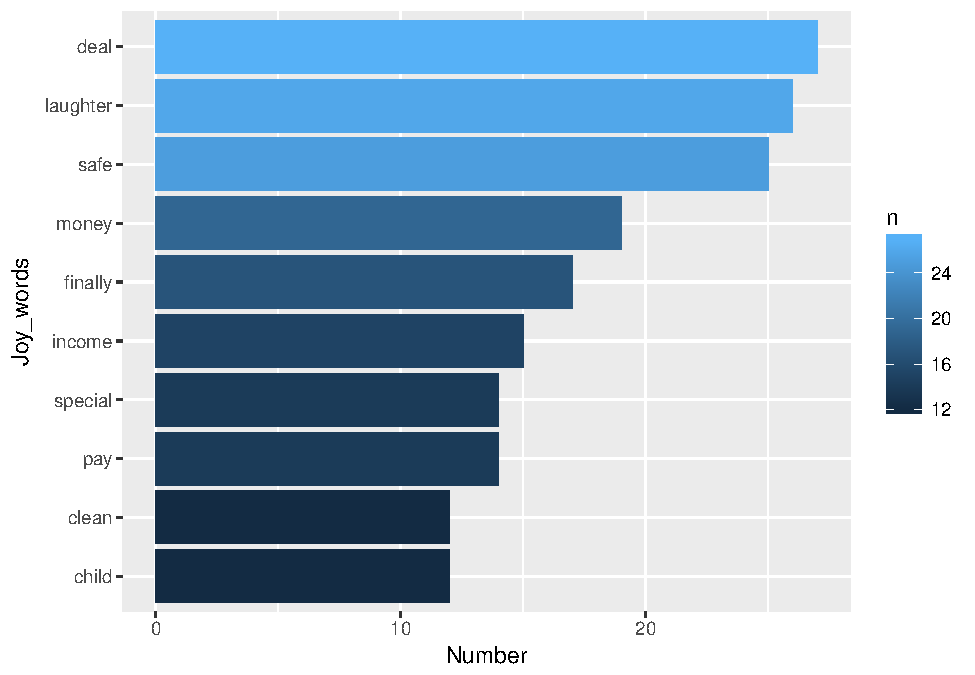
\includegraphics{Donald_Trump_Speech_sentiment_analysis_files/figure-latex/unnamed-chunk-38-1.pdf}

Now, let us see the top 10 words in Trump's speeches associated with
anticipation.

\begin{Shaded}
\begin{Highlighting}[]
\NormalTok{anticipation_trump<-Trump_sentiment}\OperatorTok\StringTok{ }\KeywordTok{inner_join}\NormalTok{(nrc_anticipation,}\DataTypeTok{by=}\StringTok{"word"}\NormalTok{)}\OperatorTok\StringTok{ }\KeywordTok{count}\NormalTok{(word)}\OperatorTok\KeywordTok{top_n}\NormalTok{(}\DecValTok{10}\NormalTok{)}
\end{Highlighting}
\end{Shaded}

\begin{verbatim}
## Selecting by n
\end{verbatim}

\begin{Shaded}
\begin{Highlighting}[]
\KeywordTok{ggplot}\NormalTok{(anticipation_trump)}\OperatorTok{+}\KeywordTok{geom_bar}\NormalTok{(}\DataTypeTok{mapping =} \KeywordTok{aes}\NormalTok{(}\KeywordTok{reorder}\NormalTok{(word,n),n,}\DataTypeTok{fill=}\NormalTok{n),}\DataTypeTok{stat =} \StringTok{"identity"}\NormalTok{)}\OperatorTok{+}\KeywordTok{coord_flip}\NormalTok{()}\OperatorTok{+}\KeywordTok{labs}\NormalTok{(}\DataTypeTok{x=}\StringTok{"anticipation_words"}\NormalTok{,}\DataTypeTok{y=}\StringTok{"Number"}\NormalTok{)}
\end{Highlighting}
\end{Shaded}

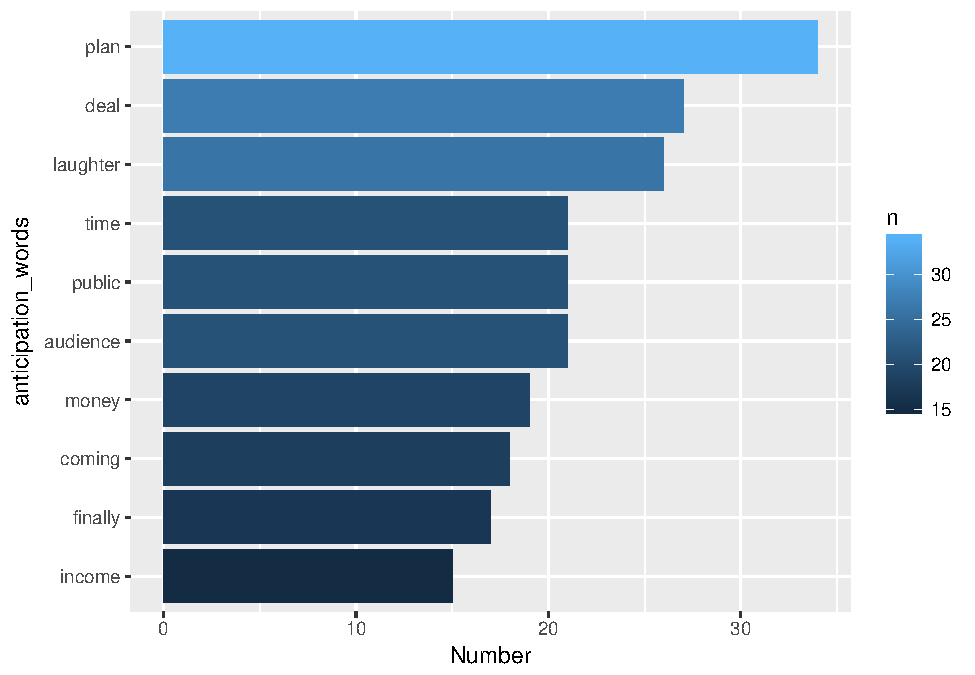
\includegraphics{Donald_Trump_Speech_sentiment_analysis_files/figure-latex/unnamed-chunk-39-1.pdf}

PART D

In this part, I will write a function to tokenize an input corpus and
spit out the most frequent words. The idea is to automate the process of
data cleansing and get a glimpse into the data at the first go.

\begin{Shaded}
\begin{Highlighting}[]
\NormalTok{Text_analysis_corpus<-}\ControlFlowTok{function}\NormalTok{(mysrc_clean,nwords)\{}
\NormalTok{  mysrc_clean<-}\KeywordTok{tm_map}\NormalTok{(mysrc_clean,removeNumbers)}
\NormalTok{  mysrc_clean<-}\KeywordTok{tm_map}\NormalTok{(mysrc_clean,removeWords,}\KeywordTok{stopwords}\NormalTok{())}
\NormalTok{  mysrc_clean<-}\KeywordTok{tm_map}\NormalTok{(mysrc_clean,removePunctuation)}
  \KeywordTok{library}\NormalTok{(SnowballC)}
\NormalTok{  mysrc_clean<-}\KeywordTok{tm_map}\NormalTok{(mysrc_clean,stripWhitespace)}
\NormalTok{ mysrc_dcm<-}\KeywordTok{DocumentTermMatrix}\NormalTok{(mysrc_clean)}

 
\NormalTok{ mysrc_sparce<-}\KeywordTok{removeSparseTerms}\NormalTok{(mysrc_dcm,.}\DecValTok{5}\NormalTok{)}
\NormalTok{mysrc_final<-}\KeywordTok{as.data.frame}\NormalTok{(}\KeywordTok{as.matrix}\NormalTok{(mysrc_sparce))}
\NormalTok{Most_common<-}\KeywordTok{colSums}\NormalTok{(Trump_final)}
\NormalTok{Top_words<-}\KeywordTok{sort}\NormalTok{(Most_common,}\DataTypeTok{decreasing =} \OtherTok{TRUE}\NormalTok{)[}\DecValTok{1}\OperatorTok{:}\NormalTok{nwords]}
\NormalTok{Word_freq<-}\KeywordTok{as.data.frame}\NormalTok{(Top_words)}


\NormalTok{Word_freq}\OperatorTok{$}\NormalTok{Word<-}\KeywordTok{rownames}\NormalTok{(Word_freq)}
\KeywordTok{rownames}\NormalTok{(Word_freq)<-}\KeywordTok{c}\NormalTok{()}
\NormalTok{Word_freq<-Word_freq[}\KeywordTok{c}\NormalTok{(}\DecValTok{2}\NormalTok{,}\DecValTok{1}\NormalTok{)]}

\KeywordTok{colnames}\NormalTok{(Word_freq)<-}\KeywordTok{c}\NormalTok{(}\StringTok{"Word"}\NormalTok{,}\StringTok{"Frequency"}\NormalTok{)}

\NormalTok{Word_freq}\OperatorTok{$}\NormalTok{Word<-}\KeywordTok{as.factor}\NormalTok{(Word_freq}\OperatorTok{$}\NormalTok{Word)}

\KeywordTok{ggplot}\NormalTok{(Word_freq)}\OperatorTok{+}\KeywordTok{geom_bar}\NormalTok{(}\DataTypeTok{mapping =} \KeywordTok{aes}\NormalTok{(}\KeywordTok{reorder}\NormalTok{(Word,Frequency),Frequency,}\DataTypeTok{fill=}\NormalTok{Frequency),}\DataTypeTok{stat =} \StringTok{"identity"}\NormalTok{)}\OperatorTok{+}\KeywordTok{coord_flip}\NormalTok{()}
\NormalTok{ \}}
\end{Highlighting}
\end{Shaded}

Let us test if the method works.

We will use the corpus from the question 6.

\begin{Shaded}
\begin{Highlighting}[]
\KeywordTok{Text_analysis_corpus}\NormalTok{(Trump_corpus,}\DecValTok{5}\NormalTok{)}
\end{Highlighting}
\end{Shaded}

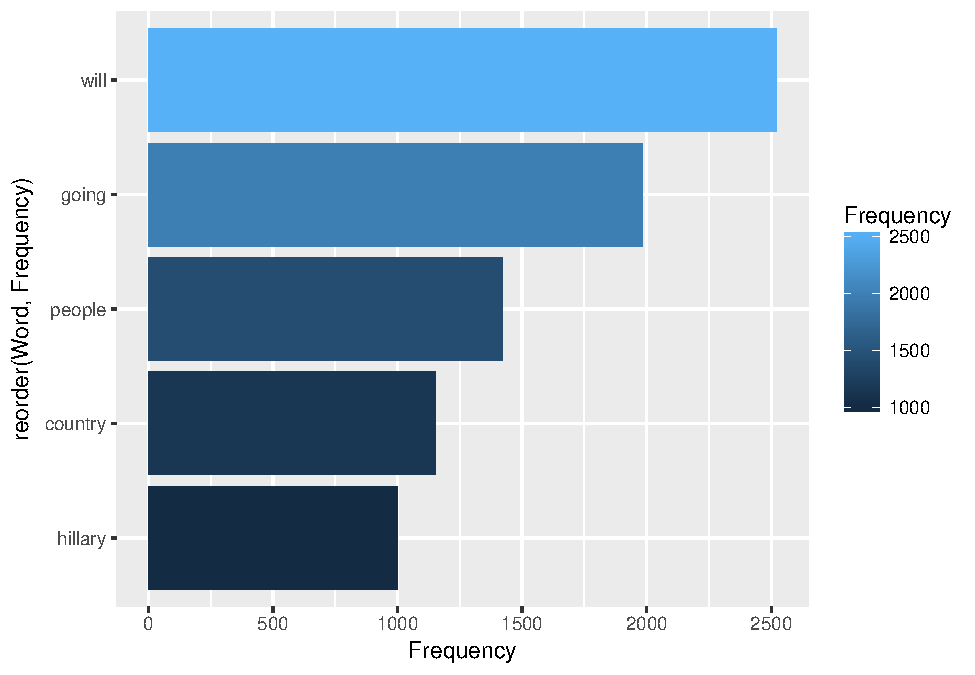
\includegraphics{Donald_Trump_Speech_sentiment_analysis_files/figure-latex/unnamed-chunk-41-1.pdf}


\end{document}
